\title{Syntax and Semantics Exam}
\author{
        Benjamin Bennetzen \\
        Student ID: 20204861 \\
        Computer Science, 4th semester\\
}
\date{\today}

\documentclass[12pt]{article}

\usepackage{tikz}
\usepackage{listings}
\usepackage{mathpartir}
\usepackage{ebproof}
\usepackage{amsmath}
\usepackage[utf8]{inputenc}
\usepackage{amssymb}
\usepackage{graphicx}
\usepackage{stmaryrd}

\newcommand{\R}{\mathbb{R}}
\newcommand{\F}{\mathbb{F}}
\newcommand{\num}[1]{\mathcal{N}\llbracket #1 \rrbracket}

\begin{document}
\maketitle

\section{Exercise}
\subsection{}

\begin{center}
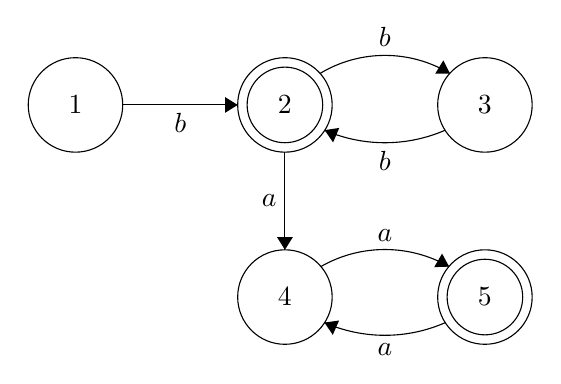
\begin{tikzpicture}[scale=0.2]
\tikzstyle{every node}+=[inner sep=0pt]
\draw [black] (13.3,-12.7) circle (3);
\draw (13.3,-12.7) node {$1$};
\draw [black] (26.6,-12.7) circle (3);
\draw (26.6,-12.7) node {$2$};
\draw [black] (26.6,-12.7) circle (2.4);
\draw [black] (39.3,-12.7) circle (3);
\draw (39.3,-12.7) node {$3$};
\draw [black] (26.6,-24.9) circle (3);
\draw (26.6,-24.9) node {$4$};
\draw [black] (39.3,-24.9) circle (3);
\draw (39.3,-24.9) node {$5$};
\draw [black] (39.3,-24.9) circle (2.4);
\draw [black] (16.3,-12.7) -- (23.6,-12.7);
\fill [black] (23.6,-12.7) -- (22.8,-12.2) -- (22.8,-13.2);
\draw (19.95,-13.2) node [below] {$b$};
\draw [black] (28.819,-10.707) arc (121.16868:58.83132:7.982);
\fill [black] (37.08,-10.71) -- (36.66,-9.87) -- (36.14,-10.72);
\draw (32.95,-9.05) node [above] {$b$};
\draw [black] (36.779,-14.304) arc (-66.49418:-113.50582:9.6);
\fill [black] (29.12,-14.3) -- (29.66,-15.08) -- (30.05,-14.16);
\draw (32.95,-15.6) node [below] {$b$};
\draw [black] (26.6,-15.7) -- (26.6,-21.9);
\fill [black] (26.6,-21.9) -- (27.1,-21.1) -- (26.1,-21.1);
\draw (26.1,-18.8) node [left] {$a$};
\draw [black] (28.873,-22.968) arc (119.85711:60.14289:8.188);
\fill [black] (37.03,-22.97) -- (36.58,-22.14) -- (36.08,-23);
\draw (32.95,-21.38) node [above] {$a$};
\draw [black] (36.79,-26.52) arc (-66.19349:-113.80651:9.513);
\fill [black] (29.11,-26.52) -- (29.64,-27.3) -- (30.04,-26.39);
\draw (32.95,-27.83) node [below] {$a$};
\end{tikzpicture}
\end{center}

\subsection{}
\begin{center}
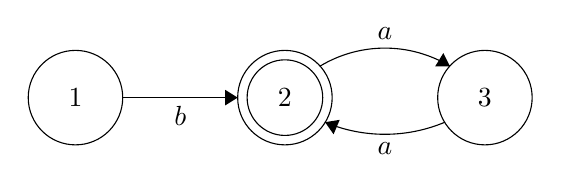
\begin{tikzpicture}[scale=0.2]
\tikzstyle{every node}+=[inner sep=0pt]
\draw [black] (13.3,-12.7) circle (3);
\draw (13.3,-12.7) node {$1$};
\draw [black] (26.6,-12.7) circle (3);
\draw (26.6,-12.7) node {$2$};
\draw [black] (26.6,-12.7) circle (2.4);
\draw [black] (39.3,-12.7) circle (3);
\draw (39.3,-12.7) node {$3$};
\draw [black] (16.3,-12.7) -- (23.6,-12.7);
\fill [black] (23.6,-12.7) -- (22.8,-12.2) -- (22.8,-13.2);
\draw (19.95,-13.2) node [below] {$b$};
\draw [black] (28.819,-10.707) arc (121.16868:58.83132:7.982);
\fill [black] (37.08,-10.71) -- (36.66,-9.87) -- (36.14,-10.72);
\draw (32.95,-9.05) node [above] {$a$};
\draw [black] (36.753,-14.263) arc (-67.2219:-112.7781:9.822);
\fill [black] (29.15,-14.26) -- (29.69,-15.03) -- (30.08,-14.11);
\draw (32.95,-15.53) node [below] {$a$};
\end{tikzpicture}
\end{center}

\subsection{}
\begin{center}
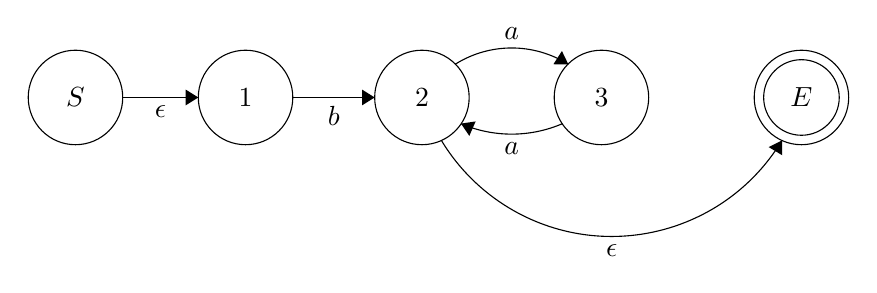
\begin{tikzpicture}[scale=0.2]
\tikzstyle{every node}+=[inner sep=0pt]
\draw [black] (22.1,-12.7) circle (3);
\draw (22.1,-12.7) node {$1$};
\draw [black] (33.3,-12.7) circle (3);
\draw (33.3,-12.7) node {$2$};
\draw [black] (44.7,-12.7) circle (3);
\draw (44.7,-12.7) node {$3$};
\draw [black] (11.3,-12.7) circle (3);
\draw (11.3,-12.7) node {$S$};
\draw [black] (57.4,-12.7) circle (3);
\draw (57.4,-12.7) node {$E$};
\draw [black] (57.4,-12.7) circle (2.4);
\draw [black] (25.1,-12.7) -- (30.3,-12.7);
\fill [black] (30.3,-12.7) -- (29.5,-12.2) -- (29.5,-13.2);
\draw (27.7,-13.2) node [below] {$b$};
\draw [black] (35.404,-10.596) arc (122.24654:57.75346:6.74);
\fill [black] (42.6,-10.6) -- (42.19,-9.75) -- (41.65,-10.59);
\draw (39,-9.06) node [above] {$a$};
\draw [black] (42.223,-14.363) arc (-66.67997:-113.32003:8.142);
\fill [black] (35.78,-14.36) -- (36.31,-15.14) -- (36.71,-14.22);
\draw (39,-15.53) node [below] {$a$};
\draw [black] (14.3,-12.7) -- (19.1,-12.7);
\fill [black] (19.1,-12.7) -- (18.3,-12.2) -- (18.3,-13.2);
\draw (16.7,-13.2) node [below] {$\epsilon$};
\draw [black] (56.165,-15.426) arc (-31.16101:-148.83899:12.639);
\fill [black] (56.17,-15.43) -- (55.32,-15.85) -- (56.18,-16.37);
\draw (45.35,-22.03) node [below] {$\epsilon$};
\end{tikzpicture}
\end{center}

\begin{center}
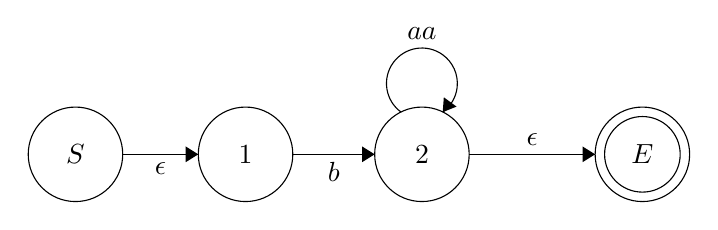
\begin{tikzpicture}[scale=0.2]
\tikzstyle{every node}+=[inner sep=0pt]
\draw [black] (22.1,-12.7) circle (3);
\draw (22.1,-12.7) node {$1$};
\draw [black] (33.3,-12.7) circle (3);
\draw (33.3,-12.7) node {$2$};
\draw [black] (11.3,-12.7) circle (3);
\draw (11.3,-12.7) node {$S$};
\draw [black] (47.3,-12.7) circle (3);
\draw (47.3,-12.7) node {$E$};
\draw [black] (47.3,-12.7) circle (2.4);
\draw [black] (25.1,-12.7) -- (30.3,-12.7);
\fill [black] (30.3,-12.7) -- (29.5,-12.2) -- (29.5,-13.2);
\draw (27.7,-13.2) node [below] {$b$};
\draw [black] (14.3,-12.7) -- (19.1,-12.7);
\fill [black] (19.1,-12.7) -- (18.3,-12.2) -- (18.3,-13.2);
\draw (16.7,-13.2) node [below] {$\epsilon$};
\draw [black] (36.3,-12.7) -- (44.3,-12.7);
\fill [black] (44.3,-12.7) -- (43.5,-12.2) -- (43.5,-13.2);
\draw (40.3,-12.2) node [above] {$\epsilon$};
\draw [black] (31.977,-10.02) arc (234:-54:2.25);
\draw (33.3,-5.45) node [above] {$aa$};
\fill [black] (34.62,-10.02) -- (35.5,-9.67) -- (34.69,-9.08);
\end{tikzpicture}
\end{center}

\begin{center}
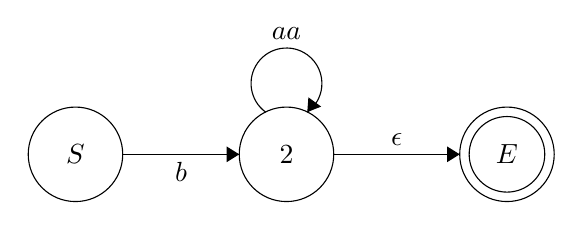
\begin{tikzpicture}[scale=0.2]
\tikzstyle{every node}+=[inner sep=0pt]
\draw [black] (33.3,-12.7) circle (3);
\draw (33.3,-12.7) node {$2$};
\draw [black] (19.9,-12.7) circle (3);
\draw (19.9,-12.7) node {$S$};
\draw [black] (47.3,-12.7) circle (3);
\draw (47.3,-12.7) node {$E$};
\draw [black] (47.3,-12.7) circle (2.4);
\draw [black] (36.3,-12.7) -- (44.3,-12.7);
\fill [black] (44.3,-12.7) -- (43.5,-12.2) -- (43.5,-13.2);
\draw (40.3,-12.2) node [above] {$\epsilon$};
\draw [black] (31.977,-10.02) arc (234:-54:2.25);
\draw (33.3,-5.45) node [above] {$aa$};
\fill [black] (34.62,-10.02) -- (35.5,-9.67) -- (34.69,-9.08);
\draw [black] (22.9,-12.7) -- (30.3,-12.7);
\fill [black] (30.3,-12.7) -- (29.5,-12.2) -- (29.5,-13.2);
\draw (26.6,-13.2) node [below] {$b$};
\end{tikzpicture}
\end{center}

\begin{center}
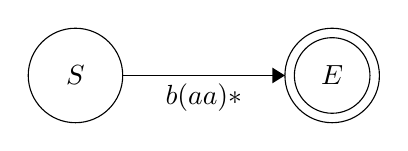
\begin{tikzpicture}[scale=0.2]
\tikzstyle{every node}+=[inner sep=0pt]
\draw [black] (31,-12.7) circle (3);
\draw (31,-12.7) node {$S$};
\draw [black] (47.3,-12.7) circle (3);
\draw (47.3,-12.7) node {$E$};
\draw [black] (47.3,-12.7) circle (2.4);
\draw [black] (34,-12.7) -- (44.3,-12.7);
\fill [black] (44.3,-12.7) -- (43.5,-12.2) -- (43.5,-13.2);
\draw (39.15,-13.2) node [below] {$b(aa)*$};
\end{tikzpicture}
\end{center}

\section{Exercise}
\subsection{}
\begin{center}
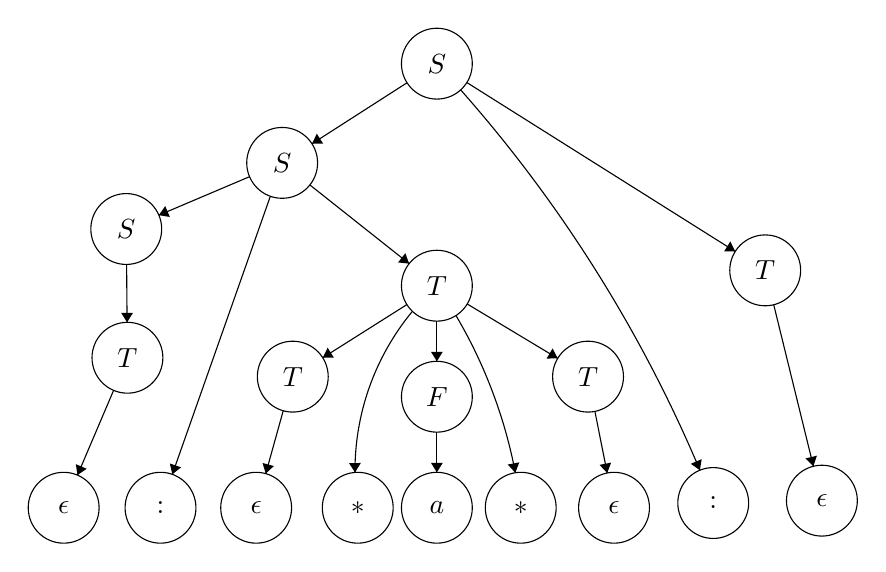
\begin{tikzpicture}[scale=0.15]
\tikzstyle{every node}+=[inner sep=0pt]
\draw [black] (36.5,-7.5) circle (3);
\draw (36.5,-7.5) node {$S$};
\draw [black] (23.4,-15.9) circle (3);
\draw (23.4,-15.9) node {$S$};
\draw [black] (10.2,-21.5) circle (3);
\draw (10.2,-21.5) node {$S$};
\draw [black] (10.3,-32.4) circle (3);
\draw (10.3,-32.4) node {$T$};
\draw [black] (4.9,-45.1) circle (3);
\draw (4.9,-45.1) node {$\epsilon$};
\draw [black] (13.1,-45.1) circle (3);
\draw (13.1,-45.1) node {$:$};
\draw [black] (36.5,-26.3) circle (3);
\draw (36.5,-26.3) node {$T$};
\draw [black] (24.3,-34) circle (3);
\draw (24.3,-34) node {$T$};
\draw [black] (49.3,-34) circle (3);
\draw (49.3,-34) node {$T$};
\draw [black] (36.5,-35.7) circle (3);
\draw (36.5,-35.7) node {$F$};
\draw [black] (21.2,-45.1) circle (3);
\draw (21.2,-45.1) node {$\epsilon$};
\draw [black] (29.8,-45.1) circle (3);
\draw (29.8,-45.1) node {$*$};
\draw [black] (36.5,-45.1) circle (3);
\draw (36.5,-45.1) node {$a$};
\draw [black] (43.6,-45.1) circle (3);
\draw (43.6,-45.1) node {$*$};
\draw [black] (51.5,-45.1) circle (3);
\draw (51.5,-45.1) node {$\epsilon$};
\draw [black] (59.9,-44.7) circle (3);
\draw (59.9,-44.7) node {$:$};
\draw [black] (69.1,-44.5) circle (3);
\draw (69.1,-44.5) node {$\epsilon$};
\draw [black] (64.3,-25) circle (3);
\draw (64.3,-25) node {$T$};
\draw [black] (33.97,-9.12) -- (25.93,-14.28);
\fill [black] (25.93,-14.28) -- (26.87,-14.27) -- (26.33,-13.43);
\draw [black] (20.64,-17.07) -- (12.96,-20.33);
\fill [black] (12.96,-20.33) -- (13.89,-20.48) -- (13.5,-19.56);
\draw [black] (10.23,-24.5) -- (10.27,-29.4);
\fill [black] (10.27,-29.4) -- (10.77,-28.6) -- (9.77,-28.6);
\draw [black] (9.13,-35.16) -- (6.07,-42.34);
\fill [black] (6.07,-42.34) -- (6.85,-41.8) -- (5.93,-41.41);
\draw [black] (22.4,-18.73) -- (14.1,-42.27);
\fill [black] (14.1,-42.27) -- (14.84,-41.68) -- (13.89,-41.35);
\draw [black] (25.75,-17.77) -- (34.15,-24.43);
\fill [black] (34.15,-24.43) -- (33.83,-23.55) -- (33.21,-24.33);
\draw [black] (33.96,-27.9) -- (26.84,-32.4);
\fill [black] (26.84,-32.4) -- (27.78,-32.39) -- (27.25,-31.55);
\draw [black] (39.07,-27.85) -- (46.73,-32.45);
\fill [black] (46.73,-32.45) -- (46.3,-31.61) -- (45.79,-32.47);
\draw [black] (36.5,-29.3) -- (36.5,-32.7);
\fill [black] (36.5,-32.7) -- (37,-31.9) -- (36,-31.9);
\draw [black] (23.49,-36.89) -- (22.01,-42.21);
\fill [black] (22.01,-42.21) -- (22.7,-41.57) -- (21.74,-41.31);
\draw [black] (29.567,-42.112) arc (-179.59697:-219.63343:21.157);
\fill [black] (29.57,-42.11) -- (30.06,-41.31) -- (29.06,-41.32);
\draw [black] (36.5,-38.7) -- (36.5,-42.1);
\fill [black] (36.5,-42.1) -- (37,-41.3) -- (36,-41.3);
\draw [black] (38.117,-28.826) arc (30.5518:10.82725:41.531);
\fill [black] (43.14,-42.14) -- (43.48,-41.26) -- (42.5,-41.44);
\draw [black] (49.88,-36.94) -- (50.92,-42.16);
\fill [black] (50.92,-42.16) -- (51.25,-41.28) -- (50.27,-41.47);
\draw [black] (38.516,-9.722) arc (41.47964:22.86279:117.589);
\fill [black] (58.77,-41.92) -- (58.92,-40.99) -- (58,-41.38);
\draw [black] (39.04,-9.1) -- (61.76,-23.4);
\fill [black] (61.76,-23.4) -- (61.35,-22.55) -- (60.82,-23.4);
\draw [black] (65.02,-27.91) -- (68.38,-41.59);
\fill [black] (68.38,-41.59) -- (68.68,-40.69) -- (67.71,-40.93);
\end{tikzpicture}
\end{center}

\subsection{}
\begin{lstlisting}
S -> T
   | S : T
T -> T * F * T
   | <empty>
F -> a
   | [ S ]
\end{lstlisting}

Add new start rule S0, which will be the new start variable.

\begin{lstlisting}
S0 -> S
S -> T
   | S : T
T -> T * F * T
   | <empty>
F -> a
   | [ S ]
\end{lstlisting}

Remove empty productions.

\begin{lstlisting}
S0 -> S
    | <empty>
S -> T
   | S : T
   | S :
   |   :
   |   : T
T -> T * F * T
   |   * F * T
   | T * F *
   |   * F *
F -> a
   | [ S ]
   | [   ]
\end{lstlisting}

Remove unit rules.

\begin{lstlisting}
S0 -> T * F * T
    |   * F * T
    | T * F *
    |   * F *
    | S : T
    | S :
    |   :
    |   : T
    | <empty>
S -> T * F * T
   |   * F * T
   | T * F *
   |   * F *
   | S : T
   | S :
   |   :
   |   : T
T -> T * F * T
   |   * F * T
   | T * F *
   |   * F *
F -> a
   | [ S ]
   | [   ]
\end{lstlisting}

Fix length of rules

\begin{lstlisting}
S0 -> T A1
    | * A2
    | T B1
    | * B2
    | S C1
    | S :
    |   :
    |   : T
    | <empty>
S -> T A1
   | * A2
   | T B1
   | * B1
   | S C1
   | S :
   |   :
   |   : T
T -> T A1
   | * A2
   | T B1
   | * B2
F -> a
   | [ D1
   | [   ]
A1 -> * A2
A2 -> F A3
A3 -> * T
B1 -> * B2
B2 -> F *
C1 -> : T
D1 -> S ]
\end{lstlisting}

Add rules for singular terminals.

\begin{lstlisting}
S0 -> T A1
    | AST A2
    | T B1
    | AST B2
    | S C1
    | S SEMI
    |   SEMI
    |   SEMI T
    | <empty>
S -> T A1
   | AST A2
   | T B1
   | AST B1
   | S C1
   | S SEMI
   |   SEMI
   |   SEMI T
T -> T A1
   | AST A2
   | T B1
   | AST B2
F -> a
   | LBRACK D1
   | LBRACK   RBRACK
A1 -> * A2
A2 -> F A3
A3 -> * T
B1 -> * B2
B2 -> F *
C1 -> : T
D1 -> S ]
AST -> *
SEMI -> :
LBRACK -> [
RBRACK -> ]
\end{lstlisting}

\subsection{}
\begin{center}
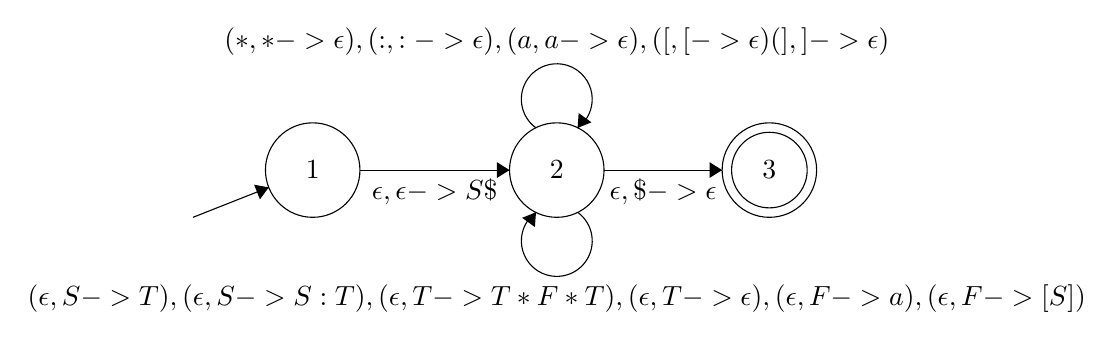
\begin{tikzpicture}[scale=0.20]
\tikzstyle{every node}+=[inner sep=0pt]
\draw [black] (19.6,-15.2) circle (3);
\draw (19.6,-15.2) node {$1$};
\draw [black] (35.1,-15.2) circle (3);
\draw (35.1,-15.2) node {$2$};
\draw [black] (48.6,-15.2) circle (3);
\draw (48.6,-15.2) node {$3$};
\draw [black] (48.6,-15.2) circle (2.4);
\draw [black] (12,-18.2) -- (16.81,-16.3);
\fill [black] (16.81,-16.3) -- (15.88,-16.13) -- (16.25,-17.06);
\draw [black] (22.6,-15.2) -- (32.1,-15.2);
\fill [black] (32.1,-15.2) -- (31.3,-14.7) -- (31.3,-15.7);
\draw (27.35,-15.7) node [below] {$\epsilon,\epsilon->S\$$};
\draw [black] (36.423,-17.88) arc (54:-234:2.25);
\draw (35.1,-22.45) node [below] {$(\epsilon,S->T),(\epsilon,S->S:T),(\epsilon,T->T*F*T),(\epsilon,T->\epsilon),(\epsilon,F->a),(\epsilon,F->[S])$};
\fill [black] (33.78,-17.88) -- (32.9,-18.23) -- (33.71,-18.82);
\draw [black] (33.777,-12.52) arc (234:-54:2.25);
\draw (35.1,-7.95) node [above] {$(*,*->\epsilon),(:,:->\epsilon),(a,a->\epsilon),([,[->\epsilon)(],]->\epsilon)$};
\fill [black] (36.42,-12.52) -- (37.3,-12.17) -- (36.49,-11.58);
\draw [black] (38.1,-15.2) -- (45.6,-15.2);
\fill [black] (45.6,-15.2) -- (44.8,-14.7) -- (44.8,-15.7);
\draw (41.85,-15.7) node [below] {$\epsilon,\$->\epsilon$};
\end{tikzpicture}
\end{center}

\section{}

\section{}
\subsection{}
\begin{equation}
   [neq-tt] \quad \frac{a_1 \rightarrow v_1 \quad a_2 \rightarrow v_2}{a_1 \neq a_2 \rightarrow tt} \quad v_1 \neq v_2
\end{equation}

\begin{equation}
   [neq-ff] \quad \frac{a_1 \rightarrow v_1 \quad a_2 \rightarrow v_2}{a_1 \neq a_2 \rightarrow ff} \quad v_1 = v_2
\end{equation}




\end{document}
